\documentclass[UTF8]{ctexart}  
\usepackage{graphicx}  
\title{HW5}
\author{王嵘晟 \quad PB1711614}
\date{}
\begin{document}
	\maketitle
	\section*{1.}
	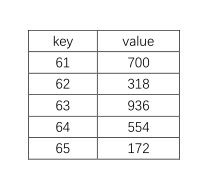
\includegraphics[scale=0.8]{1.png}
	\section*{2.}
	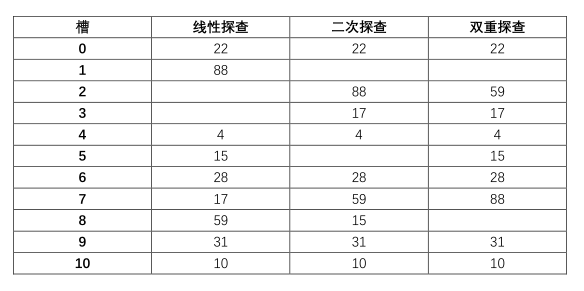
\includegraphics[scale=0.65]{2.png}
	\section*{3.}
	\par{当用中序遍历一棵二叉搜索树时,所需要的时间是$\Theta(n)$。这时输出的元素序列是按照从小到大顺序排列的。由此完成了一次从小到大对元素的排列。而如果构造一棵二叉搜索树的时间下界小于$nlgn$那么通过遍历二叉搜索树完成排序的时间复杂度就会比$nlgn$小。由此基于比较的排序中对n个元素的排序其最坏情况需要时间比$\Omega(nlgn)$小,矛盾。所以任何基于比较的算法从n个元素的任意序列中构造一棵二叉搜索树,最坏情况下需要$\Omega(nlgn)$的时间。}
	\section*{4.}
	\subsection*{4(a)}
	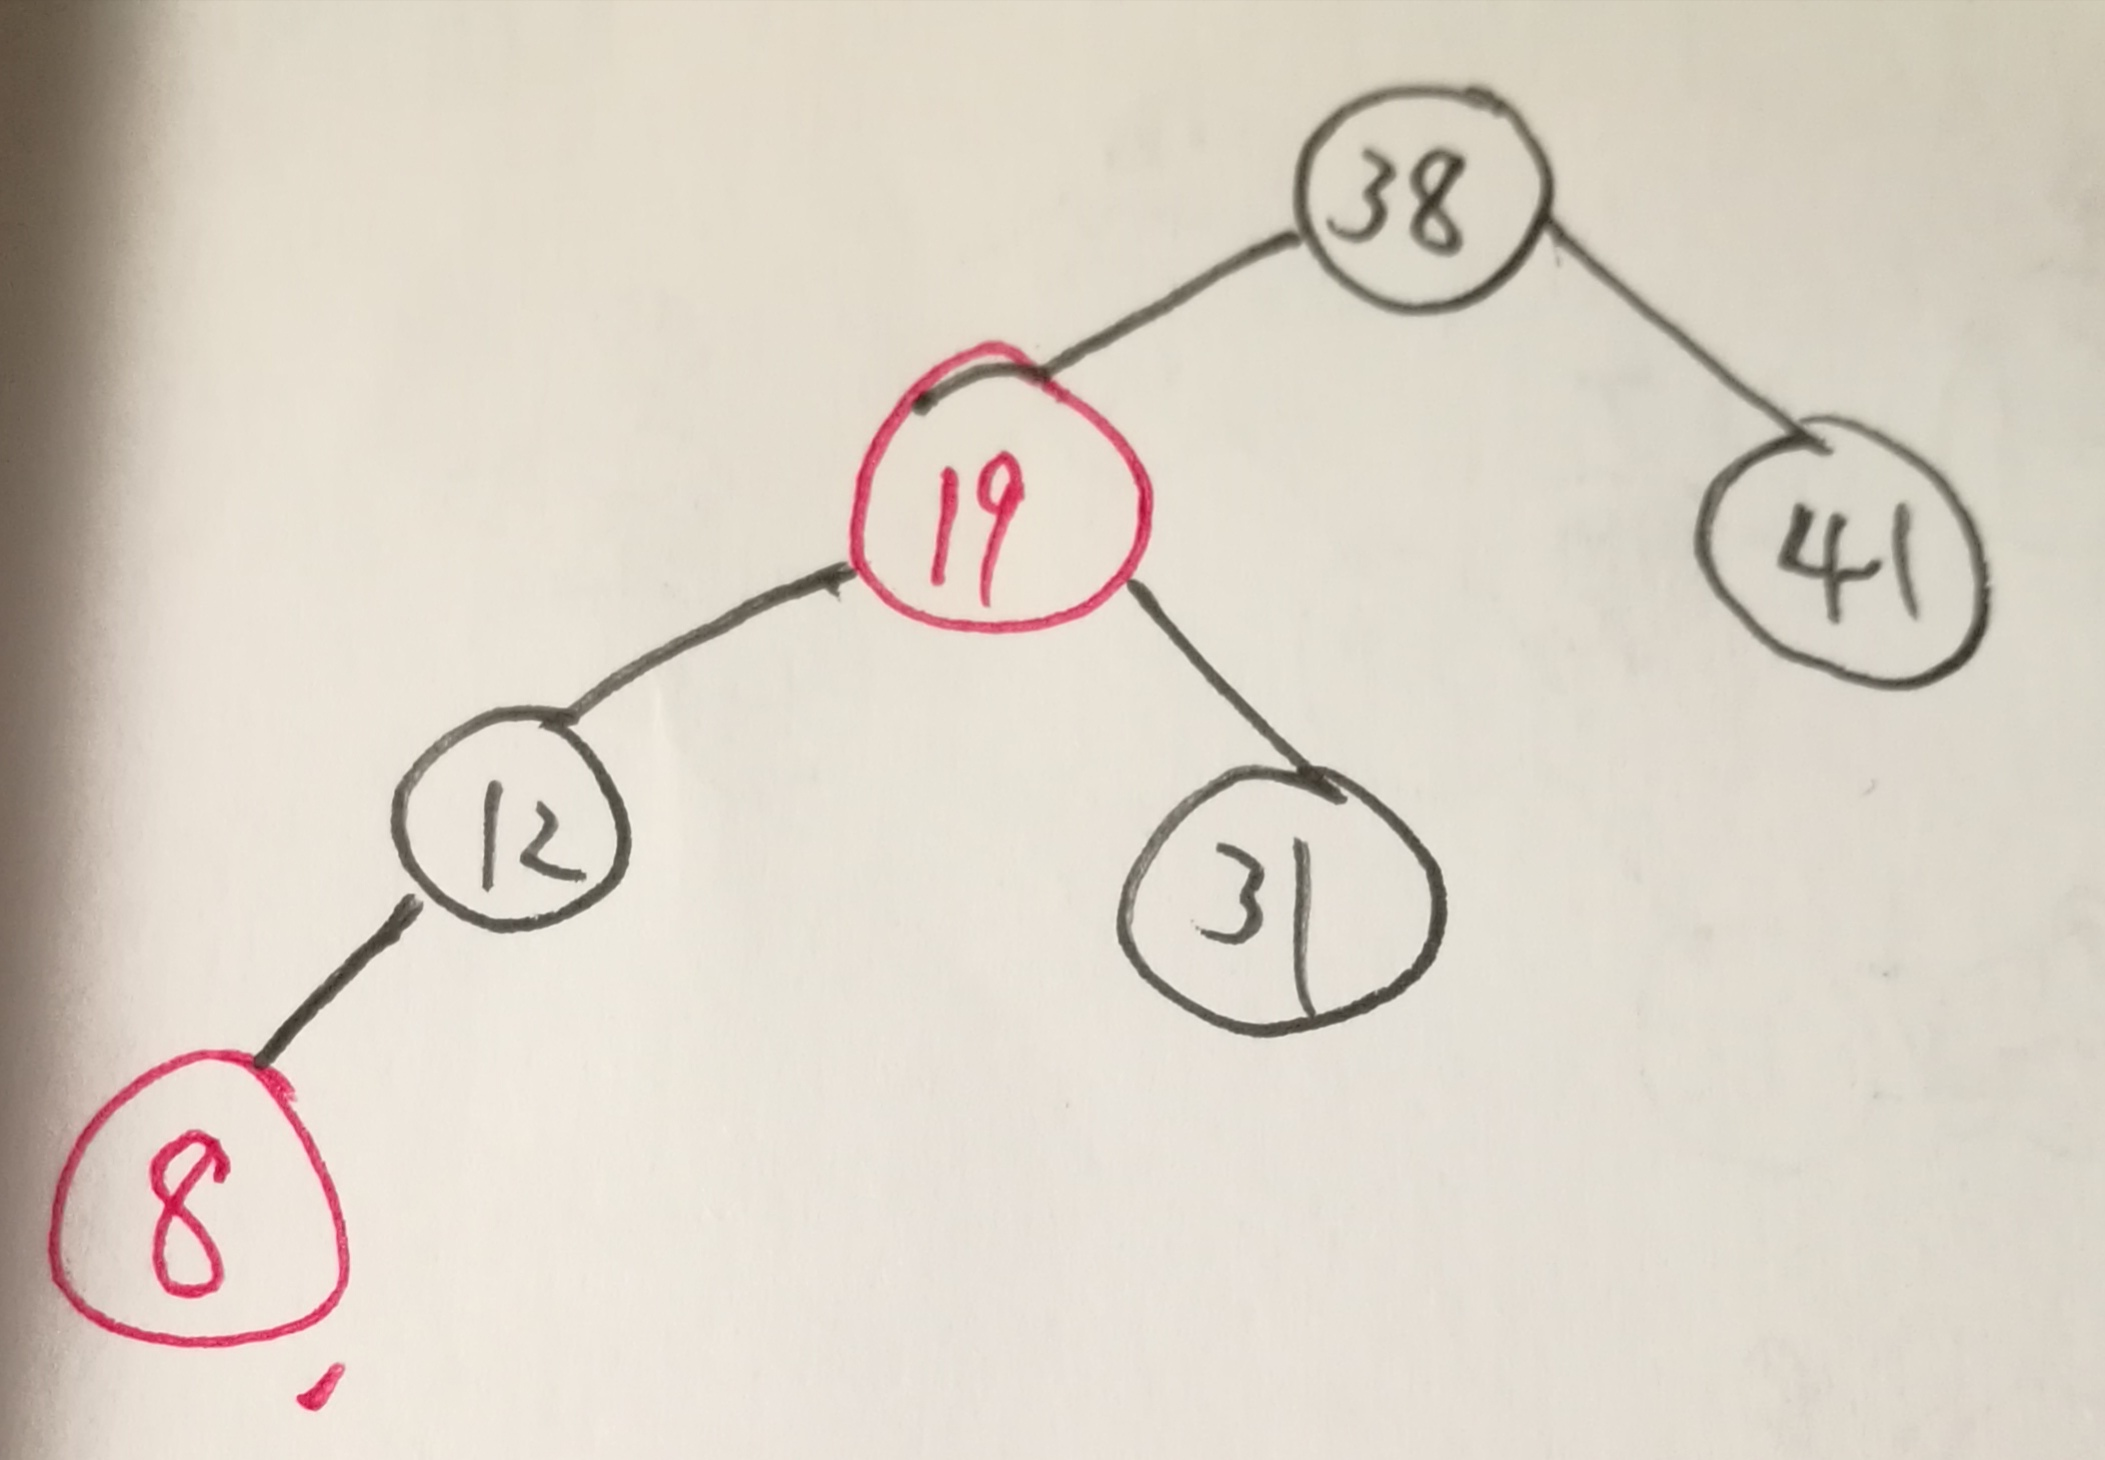
\includegraphics[scale=0.1]{1.jpg}
	\subsection*{4(b)}
	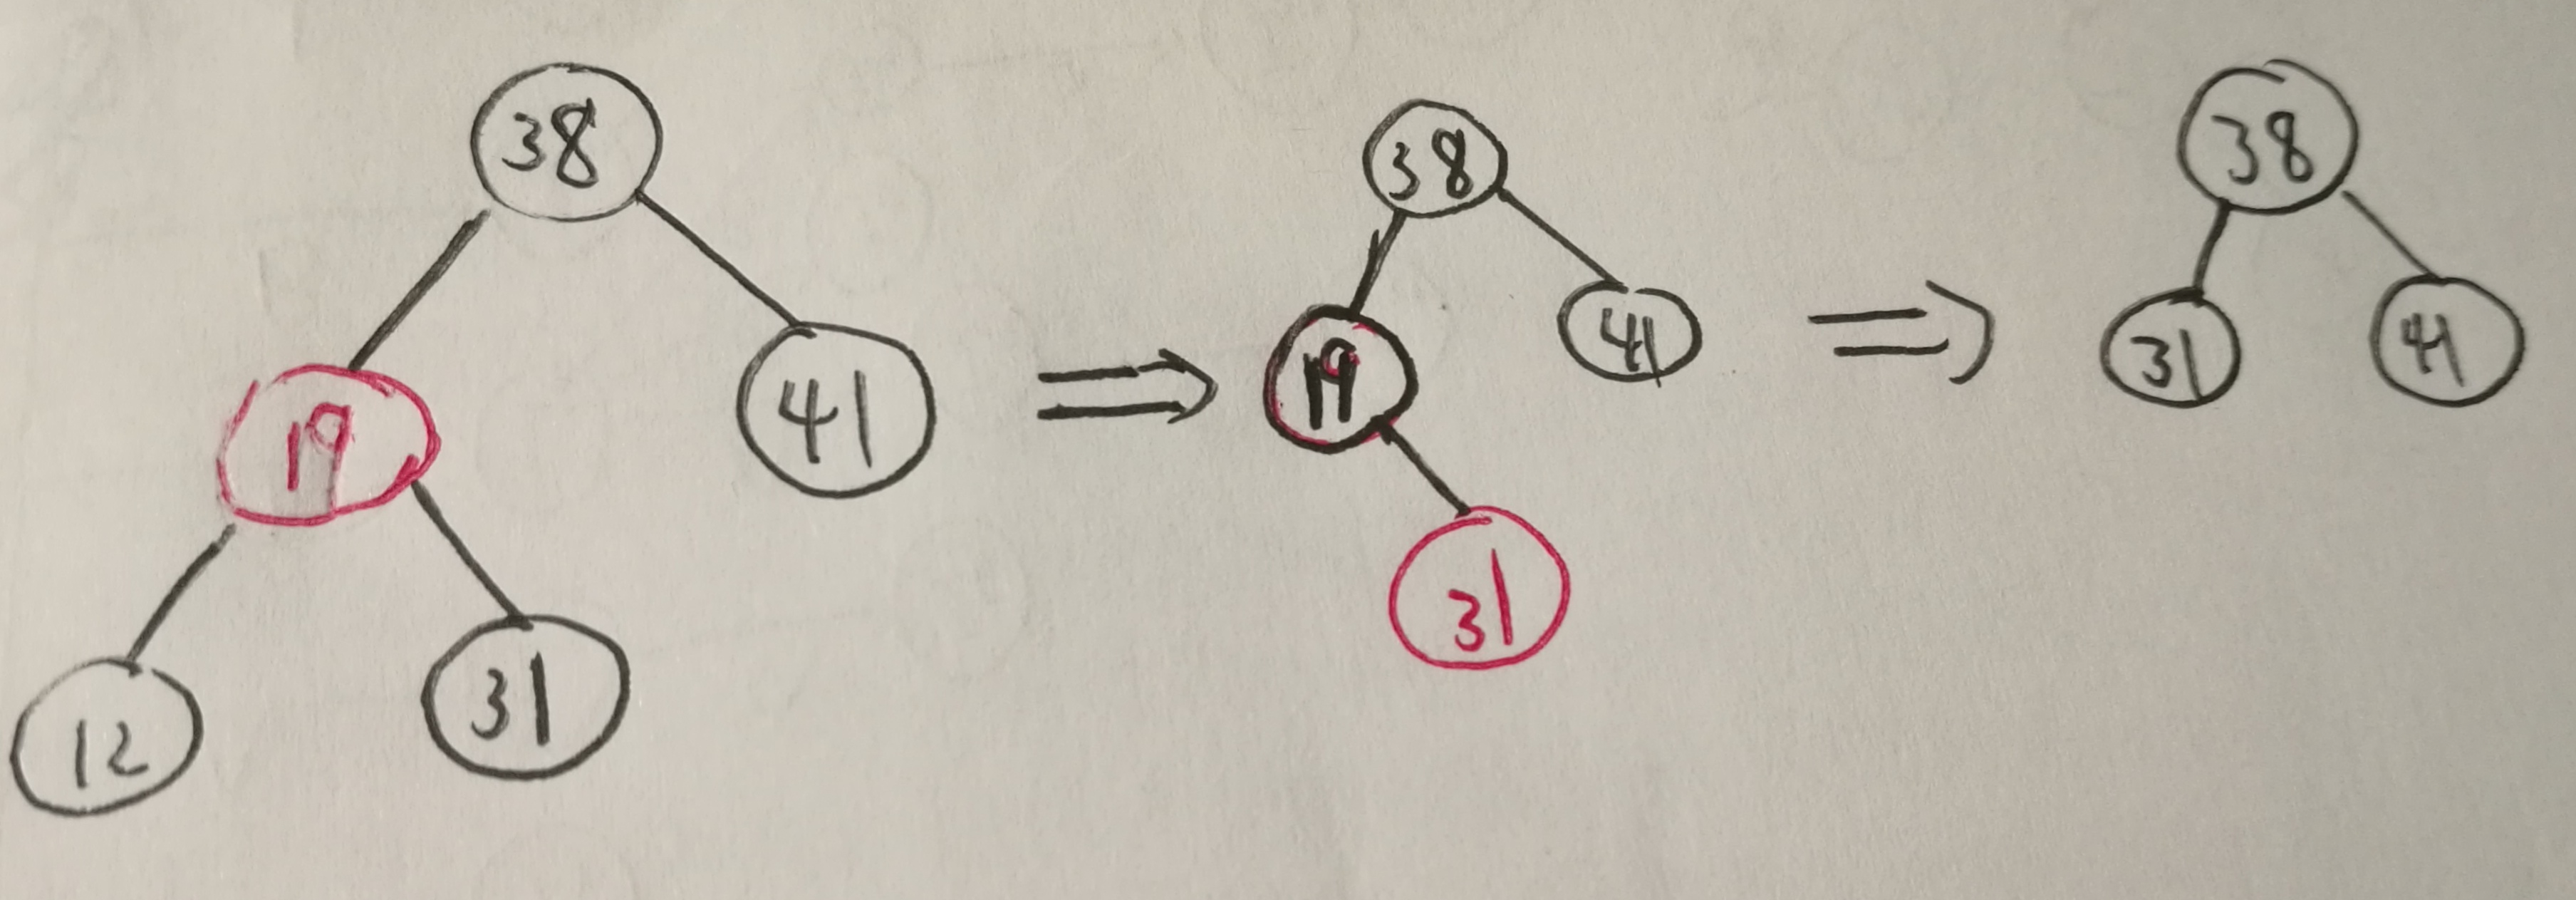
\includegraphics[scale=0.1]{2.jpg}
\end{document}